\chapter{Orígens del Bluetooth Low Energy}\label{C:compaginacio}

\section{Ús lliure de radiofreqüència}
En tot el espai radioelèctric hi ha bandes que estan assignades per a un ús privat però lliure.
Per utilitzar-les es necessari respectar la normativa nacional que normalment assimila la normativa comuna segons la ITU.
Aquestes bandes es designen ISM, acrònim de Industrial, Scientific i Medical, que són els usos pel que s'havia pensat que serviria originalment, avui en dia els usos són més diversos.

Com que l'es bandes ISM estan suficientment establertes arreu del món es crea la possibilitat per el públic general utilitzar comunicació inal·làmbrica amb molta facilitat.
Aquesta situació proporciona el disseny de productes per al consumidor habitual que ràpidament veu els avantatges de la comunicació inal·làmbrica entre dispositius.
En aquest entorn sorgeix la necessitat d'establir estàndards entre les companyies principals dels sectors corresponents.
Per definir els estàndards s'agrupen les companyies i formen grups com al WI-FI Alliance o el NFC Forum.

\section{Bluetoooth}
Bluetooth és una estàndard per l'intercanvi de dades de curt abast que utilitza la banda ISM de 2.4 GHz.
És un dels protocols més coneguts i utilitzats, sobretot a través dels dispositius mòbils.
A continuació s'explicarà l'origen d'aquesta tecnologia.

\subsection{Història de Bluetooth Clàssic}
El desenvolupament de tecnologia per a connexions de curt abast que acabarien esdevenint el que avui es coneix com a Bluetooth Clàssic va començar l'any 1989 per part de Ericsson.
Inicialment la voluntat era utilitzar aquesta tecnologia per a connectar auriculars inal·làmbrics.
D'altra banda a IBM es volia integrar connectivitat de la xarxa de telefonia als ordinadors portàtils però no era factible degut al consum d'energia que requeria la tecnologia mòbil.
IBM i Ericsson van acordar utilitzar aquesta tecnologia de curt abast en els seus productes corresponents.
El resultat va ser que els mòbils Ericsson i ordinadors ThinkPad es podrien comunicar entre si i així des del portàtil seria possible fer trucades.
Com que ni Ericsson ni IBM tenien majoria en la quota de mercat dels respectius productes van decidir que la tecnologia fos oberta.
D'aquesta manera es buscava integrar a més participants en aquesta tecnologia per tal d'estendre-la a la majoria de dispositius possibles.
El 1998 es van unir al grup Intel, Nokia i Toshiba i totes 5 companyies  van fundar el Bluetooth SIG (\textit{Bluetooth Special Interest group}, d'ara endavant SIG).
Finalment, al 2001 van sortir a la venta els primers dispositius amb Bluetooth, el terminal Ericsson T39 i el portàtil IBM ThinkPad A30.

\subsection{Història de Bluetooth Low Energy}
Com que el món de les comunicacions estava anant cap als dispositius sense fils i alimentats amb bateria, era necessari adaptar les tecnologies existents per a les noves necessitats.
L'any 2001 a Nokia es va començar a desenvolupar una versió de Bluetooth que fos similar però que reduís significativament el consum d'energia amb els compromisos mínims possibles.
Aquest desenvolupament va culminar l'any 2004 amb la publicació de la \textit{Bluetooth Low End Extension} \cite{Original_BLE_Extension}. 
Posteriorment, es va dur a terme múltiples millores juntament amb Logitech en el projecte d'investigació per part de la Unió Europea MIMOSA \cite{MIMOSA}.
El resultat del projecte es va anunciar al 2006 amb el nom de Wibree, es pot veure el logo a la figura \ref{wibree_logo}.

\begin{figure}[hb]
	\begin{center}
		
\includegraphics[width=0.6\textwidth]{./images/Wibree_Logo.png}
		\caption{Logo de Wibree}
		\label{wibree_logo}
	\end{center}
\end{figure}

Els membres del SIG després de negociar entre sí, van acordar incloure Wibree al estandard de Bluetooth en l'especificació 4.0 amb el nom de \textit{Bluetooth ultra low power technology} i publicitat com a Bluetooth Smart. El primer mòbil a incloure'l va ser el iPhone 4S al 2011.
Posteriorment es va canviar el nom per \textit{Bluetooth Low Energy} (BLE d'ara endavant)

\section{Bluetooth vs BLE}
El Bluetooth Low Energy no té cap relació amb el Bluetooth Clàssic pel que fa a l'arquitectura de la tecnologia.
Tot i que comparteixen l'ús de la banda freqüencial de 2,4 GHz, igual que altres protocols sense fils, i contenen el nom de Bluetooth queda clar que no estem parlant del mateix amb el simple fet que no son compatibles entre sí.
De fet, quant un dispositiu vol implementar les dues tecnologies (anomenat mode dual) ho ha de fer per separat ja que només comparteixen l'antena; les modulacions i altres blocs són tots diferents.

\section{MANETS (\textit{Mobile Ad-Hoc Networks})}
Bluetooth Clàssic no permet tenir més d'una connexió establerta amb dispositius.
A demés tot i voler transmetre poques dades l'arquitectura fa que es consumeixi bastanta energia per establir i mantenir la connexió.
Això no suposava problemes inicialment, ja que principalment l'ús era per la transferència de fitxers com contactes o fotografies.

Amb l'arribada dels telèfons intel·ligents, els auriculars inal·làmbrics van esdevenir populars i es va establir la dominància de Bluetooth Clàssic per a escoltar música.
Per a poder transmetre música d'alta fidelitat es va millorar Bluetooth per ser més resistent a interferències i aconseguir velocitats superiors.
Per un altre costat però va començar a sorgir el Internet of Things, basat en tenir molts dispositius connectats transmetent a taxes molt variades i de forma discontinua.
Això va generar necessitats que no es podien cobrir amb les tecnologies existents.
Era necessari tenir xarxes sense fils, amb consum molt baix d'energia i que cobrissin una gran distància (10-100 metres).
Amb aquests requeriments, van sorgir les xarxes ad hoc o \textit{Mobile Ad-Hoc Networks} (MANETS d'ara endavant).

\subsection{Altres MANETS}
BLE és una de les MANETs més importants però n'hi ha d'altres que competeixen i que s'analitzaran a continuació.

\subsubsection{Zigbee}
El estàndard Zigbee s'utilitza en entorns per a automatització de la casa, xarxes de sensors, col·lecció de dades mèdiques entre d'altres.
Zigbee està dissenyat per sobre del IEEE 802.15.4 i per tant només defineix les capes superiors.
No està pensat per a situacions amb gran mobilitat entre nodes sinó per a desplegaments més estàtics.
Zigbee s'utilitza en els dispositius de Philips Hue que serveixen per controlar bombetes intel·ligents entre d'altres.

\subsubsection{6LoWPAN}
IPv6 \textit{over Low power Wireless Personal Area Networks} és un protocol que permet enviar paquets d'Internet Protocol versió 6 a través de IEEE 802.15.4.
Aquest protocol està orientat a aportar internet amb connexions sense fils.
Una de les característiques destacades és la capacitat de comprimir les capçaleres dels paquets per així reduir el sobrecost que suposa.
La utilització de aquest protocol és majoritàriament coneguda per l'estandardització de Thread que utilitza el 6LoWPAN per a domòtica.

\subsubsection{Z-Wave}
Z-Wave és un protocol utilitzat principalment per domòtica. La comunicació es fa en una xarxa en malla que connecta els electrodomèstics i per tant permet el seu control.
La principal diferència d'aquest protocol es que utilitza únicament les freqüències ISM de la banda 800 o 900 MHz (segons continent) i així evita les interferències que hi ha a 2.4 GHz de WIFI o Bluetooth.
La utilització de freqüències més baixes permet més abast amb menys potència, especialment quant es tracta de penetrar parets.
Un exemple de dispositius que utilitzen aquesta tecnologia són els productes de la marca Ring principalment coneguts pels seus vídeo-porters intel·ligens.

\subsubsection{Insteon}
Insteon està orientat a domòtica i utilitza conjuntament radiofreqüència i les línies d'alimentació de casa per a la comunicació.
Aquest tipus de sistema s'anomena de malla dual.
El fet d'estar connectats tots els dispositius a la instal·lació elèctrica permet molt bona sincronització entre els dispositius.
Això permet, per exemple, que múltiples dispositius puguin retransmetre paquets alhora per tal de millorar la cobertura i reduir les retransmissions.
SmartLabs és la companyia que fabrica i ven els productes que utilitzen Insteon.
La tecnologia és pot controlar a través de Cortana, Alexa o Apple Watch entre d'altres.

\subsubsection{LoRa}
El Long Range desenvolupat per Semtech està orientat a cobrir les distàncies més grans d'entre les MANETs.
Ho aconsegueix reduint la tassa de transmissió de dades reals així augmentant el temps dedicat a cada símbol donant més oportunitats al receptor per detectar correctament el senyal.
Aquesta tècnica s'anomena espectre eixamplat i LoRa la implementa amb \textit{Chirps}.
Els \textit{Chirps} són polsos que es transmeten, s'envien més \textit{Chirps} que bits i la relació ve definida pel factor d'eixamplat o \textit{Spreading Factor}.
LoRa permet configurar aquest paràmetre que defineix l'equilibri entre la tassa de dades i la distància, pot prendre valors entre 7 i 12.
El LoRa també implementa protecció contra errors o FEC (\textit{Forward Error Correction}) per incrementar encara més el abast.

LoRa defineix les capes inferiors, la LoRa Alliance va definir el LoRaWAN que és un dels protocols que es poden utilitzar per a les capes superiors. El LoRaWAN està basat en un Control d'Accés al Medi (MAC en anglès).


\subsection{Comparació}
Tot i que els protocols tenen molt en comú cada un es diferencia de la resta en els detalls, a continuació veiem una comparació de les capacitats de cada un dels protocols

\begin{table}[!h]
	\centering
	\resizebox{\textwidth}{!}{
		\begin{tabular}{|r|c|c|c|c|c|c|c|}
			\hline
			    & BLE 4                                                  & BLE 5   & 6LoWPAN & Zigbee      & Z-Wave      & Insteon & LoRa            \\ \hline
			Abast (m)               & 50                                                     & 200     & 100     & 100         & 90          & 120     & 10Km            \\	\hline
			Velocitat Física (Kbps) & 1000                                                   & 2000    & 250     & 250         & 100         & 4,5     & 27              \\	\hline
			Tasa de dades (Kbps)    &	800 & 1430    & 162     & 162         & 40          & 2,8     & 5               \\	\hline
			Consum                  & 15                                                     & 15      & 15      & 30          & 23          &         & 18              \\	\hline
			Banda                   & 2.4                                                 & 2.4  & 800-900 i 2.4      & 800-900 i 2.4 & 800-900 & 915 & 400/800-900	\\	\hline
		\end{tabular}
	}
\caption{Comparació entre MANETs}
\end{table}

Tal i com s'ha vist BLE és classifica segons les seves capacitats en la seva versió 4 i en la 5. En el següent apartat es veurà perquè és així.


\section{Versions de BLE}
\label{Versions_BLE}
En quant al estàndard Bluetooth Low Energy cal diferenciar les característiques de la versió 4.0 amb la 5 ja que hi ha canvis significatius \cite{BLE_5_improvement_over_4}.

\subsubsection{LE 2M}
LE2M (\textit{Low Energy 2 Mega}) és el nom que te la nova capa física quan opera a 2 MBd\footnote{Baud: Unitat de mesura de la velocitat de modulació, que correspon al nombre de canvis de l'estat d'un senyal en un segon \cite{Baud_definition}.} en la versió 5 enlloc dels 1 MBd que es podia anteriorment en la versió 4.0.
L'augment de la velocitat dels símbols permet augmentar la quantitat de dades que es poden transmetre a nivell d'aplicació.
Aquest canvi està pensat per facilitar la utilització de BLE en situacions més exigents pel que fa a volum de dades com per exemple múltiples mesures del cos humà.

\subsubsection{Abast}
Tot i que la tecnologia BLE ja de per si en la seva versió original (4.0) tenia una distància màxima de transmissió teòrica molt gran (100 metres sense obstacles), no era suficient per a tots els casos.
Per exemple, era necessari tenir més abast en els sectors com el de les cases intel·ligents.
El límit de l'abast ve definit per la potència màxima de transmissió (sigui per protocol o per normativa) i per la probabilitat d'error de bit BER (\textit{Bit Error Ratio}) que es pot acceptar.
Bluetooth defineix la BER màxima en 0.1\% per tant quant un de cada mil bits és erroni es considera que la connexió és massa dolenta i que ja s'ha arribat al límit de distància.

Per tractar els errors en transmissió hi ha dues estratègies: detecció d'errors i correcció d'errors.
En la versió 4.0 de Bluetooth només s'utilitzava la detecció d'errors.
En Bluetooth 5 s'implementa correcció d'errors d'aquesta manera sense augmentar la potència transmesa es pot incrementar el abast màxim que pot tenir la comunicació.
El desavantatge és que més bits dels que es transmeten es dediquen a corregir errors per tant queda menys espai per a dades de l'aplicació.


El esquema de correcció d'errors (\textit{Forward Error Correction}) es fa amb un codificador convolucional que pot generar a la sortida més bits dels que entren. El codificador pot funcionar amb dos esquemes diferents s'anomenen $S=2$ i $S=8$.
Amb els diferents esquemes s'utilitza una taxa de codi diferent que pot augmentar la capacitat de correcció i incrementar el abast però disminuir la quantitat de dades que es poden transmetre.
Es poden veure les diferents esquemes a la taula \ref{FEC} 

\begin{table}[htb]
	\begin{center}
		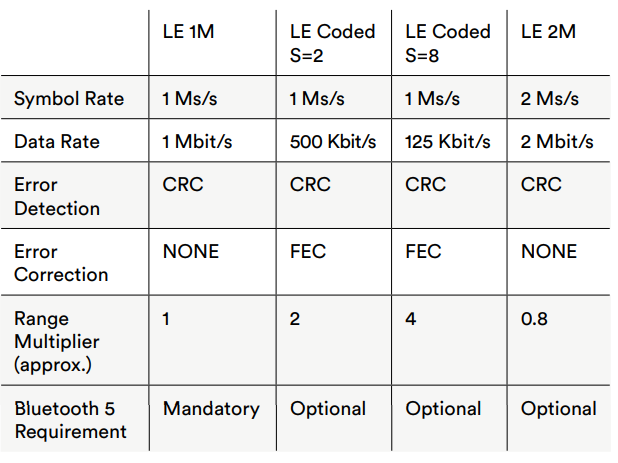
\includegraphics[width=0.8\textwidth]{./images/LE_PHY.png}
		\caption{Comparació de diferents capes físiques}
		\label{FEC}
	\end{center}
\end{table}

\subsubsection{Advertisement Extensions}
\label{Advertisement_Extensions}
En Bluetooth 4.0 els paquets d'anunci (\textit{Advertisement Packets}) tenen 6 octets de capçalera i com a molt 31 de dades, és a dir, com a molt es poden transmetre 31 Bytes de cop.
Normalment aquests paquets es transmeten pels 3 canals d'anuncis el 37, 38 i 39.

En Bluetooth 5 per poder difondre (\textit{broadcast}) més dades el que es fa és enviar un paquet d'anunci on només s'indica la capçalera i un punter cap al canal per on s'enviarà el paquet complet.
Posteriorment, pel canal per on s'ha indicat s'envia el paquet de dades i en cas de necessitar més dades s'encadenen paquets.
I d'aquesta manera les dades només es transmeten una vegada ja que abans, calia transmetre-les en els tres canals d'anunci.
Aquest procediment està detallat més endavant en l'apartat  \ref{Advertising_Extension_PDU}

En la versió 4.0 sempre hi havia una component aleatòria que marcava en quin moment s'enviava el paquet, això és comú i serveix per evitar col·lisions periòdiques.
El problema que genera és que les ràdios han d'estar més temps escoltant fins a rebre el paquet per culpa d'aquesta aleatorietat.

En BLE 5 el GAP defineix un mode síncron que permet establir un procediment d'establiment de paquets anunci sincronitzats.
Existeix una nova capçalera (SyncInfo) on s'indica amb exactitud el interval i variació (per evitar col·lisions) dels paquets.    

\subsubsection{Slot Availability Masks}
La tecnologia LTE (telefonia) està utilitzant cada vegada més espai freqüencial i en preparació de que s'utilitzi en freqüencials pròximes a la banda de 2.4 GHz ISM s'ha desenvolupat un sistema per indicar disponibilitat en el temps.
Per evitar les possibles interferències que causin altres tecnologies es defineix la SAM (\textit{Slot Availability Mask}) que permet identificar aquelles ranures de temps hi ha disponibilitat així bloquejant aquells moments on hi hagui interferències i així evitar-les.

\subsubsection{Improved Frequency Hopping}
Els salts en freqüència que utilitza la versió 4.0 estan definit per 12 seqüències predeterminades.
En BLE 5 s'utilitza una seqüència pseudo-aleatòria per determinar quins canals s'utilitzen. El algorisme en aquest cas \textit{channel selection algorithm \#2} i és més efectiu a evitar interferències i esvaniments per propagació multi-camí.

\section{Pila BLE}
Un cop vistes les característiques generals del protocol cal entendre com funciona per dins.
En entrar en detall queda clar com el protocol s'ha dissenyat de forma molt flexible.

\begin{figure}[h!]
	\begin{center}
		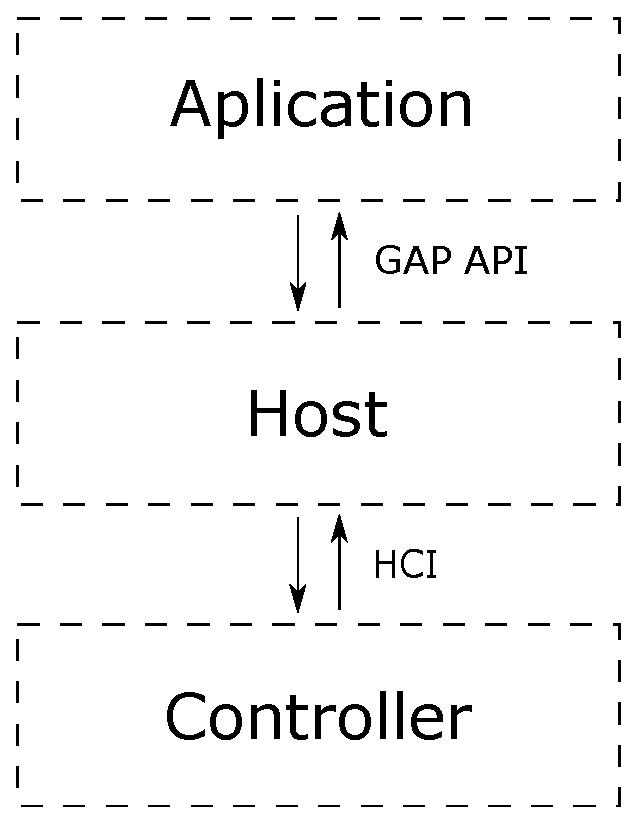
\includegraphics[width=0.4\textwidth]{./diagrames/BLE_Stack_Simplified}
		\caption{Pila de BLE}
		\label{ble_stack}
	\end{center}
\end{figure}

La pila pròpia de Bluetooth Low Energy està dividida en dues parts, tal i com es pot veure a la figura \ref{ble_stack}, el controlador i el \textit{host}. Aquestes dues parts són independents i utilitzen el protocol \textit{Host Controller Interface} (HCI d'ara endavant) per comunicar-se entre si.
Aquest protocol pot estar implementat amb qualsevol protocol de transport físic com USB o UART.
La idea darrera separar la pila en dos serveix per fer compatible xips fets per diferents fabricants.
Les dues parts de la pila poden estar implementades en el mateix xip anomenat configuració única o en xips separats anomenat configuració dual.


\subsection{Controller}
El controlador compren la capa física i la capa d'enllaç.

\begin{figure}[h!]
	\begin{center}
		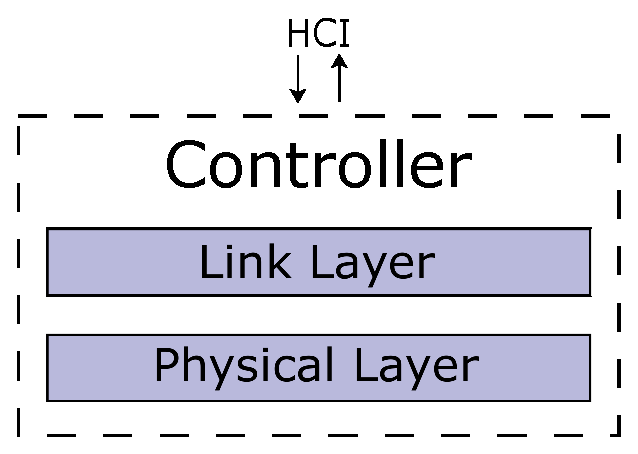
\includegraphics[width=0.4\textwidth]{./diagrames/BLE_Controller}
		\caption{Controller Stack}
	\end{center}
\end{figure}

\subsubsection{Capa Física}
La capa física és la que s'encarrega de la comunicació anal·lògica modulant i desmodulant les senyals.
Tal i com ja s'ha comentat abans treballa a la banda de 2.4 GHz en 40 canals diferents tal i com es mostra a la figura \ref{BLE_Channels}.

\begin{figure}[hb]
	\begin{center}
		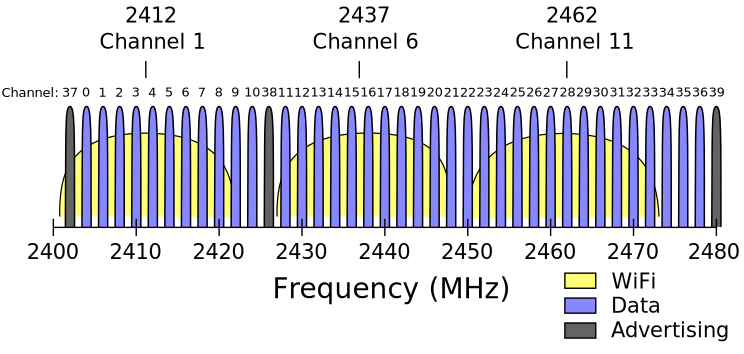
\includegraphics[width=0.8\textwidth]{./diagrames/BLE_WiFi}
		\caption{Canals BLE}
		\label{BLE_Channels}
	\end{center}
\end{figure}

Els canals es classifiquen es divideixen en 37 de dades o també anomenats secundaris i 3 d'anunci (\textit{Advertisment} o primaris).
En els canals d'anunci es vol tenir més qualitat ja que la informació que s'hi transmet és més important.
Per exemple, són els canals que s'utilitzen per descobrir altres dispositius.
És per això, que els canals d'anunci es troben en el buits que deixen els canals WiFi més comuns (1, 6 i 11), es pot veure a la figura \ref{BLE_Channels}.

El protocol BLE està orientat a consumir el mínim d'energia possible i això s'aconsegueix, principalment, reduint el temps que s'està transmitent o escoltant a través de la ràdio.
Si no s'ha de rebre o transmetre res, es pot apagar la ràdio i s'estalvia energia.
La manera de tenir apagada la ràdio més temps és transmetre les dades el més ràpid possible.
BLE és dels protocols que tenen la tassa de transmissió física \footnote{La tassa de transmissió física és aquella a la que transmeten la ràdio, no confondre amb la tassa de dades d'aplicació \textit{Throughput}} més alta, de fins a 1 Mbps originalment i de 2 Mbps en BLE 5.

La potencia de transmissió de la ràdio es pot controlar, disminuint-la per consumir menys energia.
La potència màxima és de 10 dBm (10 mW) segons la especificació\footnote{La placa utilitzada pot transmetre fins a 5 dBm de potència}.
Això serà possible sempre que l'entorn ho permeti i el receptor pugui rebre el senyal correctament.
El paquets de BLE indiquen la potència amb que s'han transmès i junt amb el RSSI (\textit{Received Signal Strength Indicator}), la potència rebuda, es pot estimar la distància fins al transmissor.
Conèixer aquest valor és útil per a certes aplicacions, per exemple, localització en espais interiors.

La modulació utilitzada per BLE és la GFSK (\textit{Gaussian Frequency Shift Keying}), la mateixa que la majoria de MANETS que es basen en el IEEE 802.11.
Aquesta modulació és una de les més robustes, simples d'implementar i és el que permet, en part, a BLE tenir un abast molt més gran que Bluetooth Clàssic.
El filtre gaussià redueix el consum pic d'energia \cite{BLE_Review} i també redueix les interferències en freqüències veïnes.
En BLE 4.0 s'utilitza una desviació freqüencial de 185 kHz, en BLE 5 com que augmenta la velocitat de símbols també creix la interferència intersimbòlica.
Per mitigar aquest efecte negatiu la desviació de freqüència passa a ser de 370 kHz.


\subsubsection{Link Layer}
La capa d'enllaç és la encarregada d'escanejar, anunciar i gestionar connexions amb altres dispositius.

Depenent d'el moment en la connexió els dispositius estan en diferents estats.
Els estats son: Espera (\textit{Idle}), Anunciador (\textit{Advertiser}) o Escàner (\textit{Scanner}) i Iniciador (\textit{Initiator}), Esclau (\textit{Slave}) o Mestre (\textit{Master}).
A la figura \ref{Link_State_Diagram} s'hi pot veure el flux d'estats per arribar a ua connexió.

\begin{figure}[!h]
	\begin{center}
		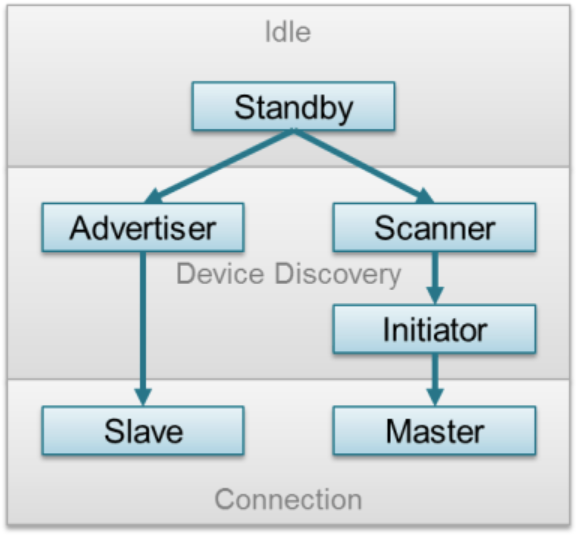
\includegraphics[width=0.5\textwidth]{./images/gap_state_diagram.png}
		\caption{Estats de la capa d'enllaç \cite{Link_Layer_states}}
		\label{Link_State_Diagram}
	\end{center}
\end{figure}

Per mitigar l'efecte de les interferències el protocol utilitza salt en freqüència (\textit{frequency hopping}).
Això permet reduir l'impacte d'una interferència estreta.
Si s'utilitzes només un dels canals BLE i en aquell canal hi haguessin interferències no es podria establir comunicació.
Al alternar múltiples canals, encara que hi hagui interferències en algun d'ells es considera que no n'hi haurà en tots i per tant hi podrà haver una comunicació bona.
Els salts que es fan són des de 5 fins 16 canals per salt d'entre els dedicats a dades.

%Bluetooth també permet la implementació de salts en freqüència adaptatius on només s'utilitzen canals suficientment bons descartant aquells en que es considera que hi ha masses interferències.

\subsection{Host}
	\begin{figure}[h!]
		\begin{center}
			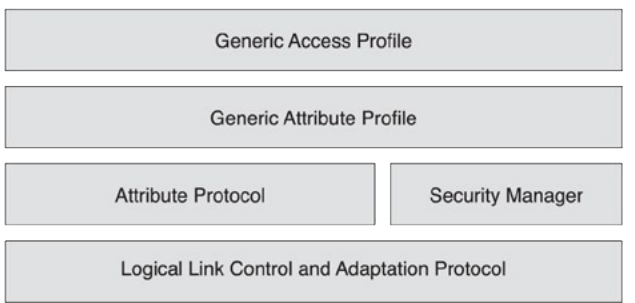
\includegraphics[width=0.6\textwidth]{./images/host.png}
			\caption{Pila del Host}
	\end{center}
\end{figure}

\subsubsection{L2CAP (\textit{Logical Link Control and Adaptation Protocol})}
La \textit{Logical Link Control and Adaptation Protocol} és la capa encarregada de l'establiment de la connexió lògica, multiplexament de protocols, segmentació i 'reasembly', control de flux per canal.

La multiplexació de protocols és necessària per aconseguir que BLE sigui flexible.
Permet que des de capes superiors s'utilitzin els protocols que es vulguin i no només aquells determinats pel estàndard de BLE.

Per limitació física de l'arquitectura existeix una MTU\footnote{La MTU és la mida màxima que pot tenir un paquet} (\textit{Maximum Transmission Unit}) i per tant els paquets de les capes superiors es converteixen en paquets més petits per a les capes inferiors.
Aquesta MTU es pot definir per cada connexió així flexibilitzant la manera que s'utilitza el protocol per a cada cas.

La L2CAP també és la capa que fa el seguiment de la qualitat de la connexió i dels recursos utilitzats per assegurar-se que les necessitats dels serveis es compleixen.

\subsubsection{SMP}
La capa \textit{Security Management Protocol} proveeix de diferents serveis relacionats amb la seguretat de la connexió.
Aquests serveis són: autenticació i autorització de dispositius i també integritat, confidencialitat i privacitat de les dades.
El protocol té tipus d'emparellament i generació de claus flexible per aconseguir reduir els requeriments de memòria i energia.
Es comentarà en més profunditat a l'apartat \ref{sec:security}

\subsubsection{ATT \& GATT}
El \textit{Attribute Protocol} (ATT d'ara endavant) és el protocol d'aplicació més comú per a BLE i el \textit{Generic Attribute Profile} defineix com utilitzar el protocol per oferir serveis a capes superiors.
El ATT és un protocol dissenyat per a dispositius \textit{Low Energy} amb l'objectiu de minimitzar la quantitat de dades transmeses. El atribut està format per 4 elements, \textit{handle}, UUID, permisos  i \textit{value}.

El \textit{handle} fa la distinció única entre els diferents atributs, ocupa 16 bits i és comú que siguin valors seqüencials però no obligatori. És molt útil ja que s'utilitza per referenciar el atribut amb el mínim de bits possibles.
El UUID (\textit{Universal Unique IDentifier}) identifica el tipus d'atribut, aquest numero pot ser de 16 bits si s'utilitza algun que ja estandarditzat pel SIG o bé en tindrà 128 bits si està definit pel fabricant.
En els permisos s'indicarà quin tipus d'accés té el client a la informació (només lectura, lectura i escriptura ...). També pot estar definit si requereix un nivell mínim d'encriptació o si es necessari l'autenticació.
Per últim el valor del atribut serà on hi ha la informació, la seva interpretació i longitud (512 bytes com a molt) dependrà del UUID.

Des del punt de vista del GATT els dispositius són clients i servidors, normalment el client pren la iniciativa demanant dades però el servidor també te la capacitat d'iniciar una comunicació per exemple notificant quan un valor ha canviat.
%TODO referenciar l'explicació en detall

La definició del ATT és massa genèrica per si sola tal que seria comú que per fer el mateix es desenvolupessin múltiples definicions que fossin incompatibles entre sí.
Per tal de tenir millor definits els serveis s'utilitza el GATT.
El GATT permet definir perfils que agrupen múltiples atributs en un sol servei \cite{services} tal i com es mostra en la figura \ref{fig:Gatt_Hierarchy}.

\begin{figure}[h!]
	\begin{center}
		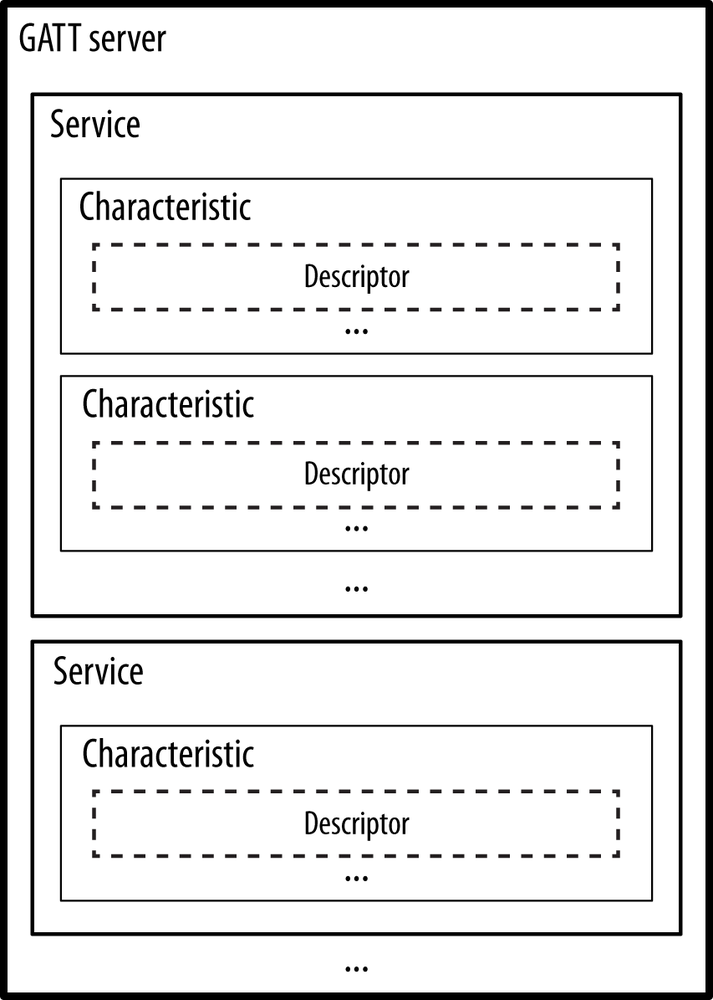
\includegraphics[width=0.4\textwidth]{./images/GATT_Hierarchy.png}
		\caption{Jerarquia de GATT \cite{GATT_Hierarchy}}
		\label{fig:Gatt_Hierarchy}
	\end{center}
\end{figure}

En un llistat de atributs el GATT identifica els serveis tenint en compte que cada servei comença amb un atribut amb el UUID 0x2800.
Aquest atribut amb UUID 0x2800 s'anomena Declaració de Servei i tots els atributs consecutius fins a una altre declaració de servei formen part d'aquest.
En la declaració de servei el camp ``valor'' indica el UUID que identifica de quin servei es tracta.

Cada servei conté característiques \cite{characteristics} definides en els atributs amb UUID 0x2803.
Aquests tipus atributs s'anomenen Declaració de Característica.
El valor de la declaració de característica està format per un nou UUID que identifica la característica i per un \textit{handle}.
Aquest \textit{handle} correspon al atribut on hi ha les dades de la característica.

\begin{table}[h]
	\begin{center}
		\definecolor{lightred}{RGB}{255, 128, 128}
		\definecolor{lightyellow}{RGB}{238, 232, 170}
		\begin{tabular}{|l|l|l|l|}
			\hline
			Handle	&	UUID	&	Descripció						&	Valor		\\ 	\hline \rowcolor{lightred}
			0x0100	&	0x2800	&	Battery Service					&	UUID 0x180F	\\		\hline \rowcolor{lightyellow}
			0x0101	&	0x2803	&	Characteristic: Battery Level	&	\parbox[t]{4cm}{UUID 0x2A19	\\ Value handle: 0x0102}	\\	\hline
			0x0102	&	0x2A2B	&	Battery Value					&	20	\\	\hline	\rowcolor{lightred}
			0x0103	&	0x2800	&	Custom Temperature Service		&	UUID 	706676c8-3e49...	\\	\hline	\rowcolor{lightyellow}
			0x0104	&	0x2803	&	Characteristic: Temperature		&	\parbox[t]{4cm}{UUID 0x2A6E	\\ Value handle: 0x0105}	\\		\hline	
			0x0105	&	0x2A6E	&	Temperature Value				&	25.45	\\	\hline \rowcolor{lightyellow}
			0x0106	&	0x2803	&	Characteristic: date/time		&	\parbox[t]{4cm}{UUID 0x2A08	\\ Value handle: 0x0107}	\\		\hline
			0x0107	&	0x2A08	&	Date/Time						&	1/1/1980 12:00	\\
			\hline
		\end{tabular}	
		\caption{Exemple de possibles atributs}
		\label{Attribute_Table}
	\end{center}
\end{table}

En aquest exemple de la taula \ref{Attribute_Table} es pot veure que hi ha 2 serveis diferents, marcats en vermell, ja que hi ha 2 UUIDs 0x2800.
També hi ha 3 característiques en total, marcades en groc, (una pel primer servei i dues pel segon) ja que hi ha 3 atributs amb UUID 0x2803.
Com que els valors corresponents al nivell de bateria i la temperatura estan estandarditzats (veure \cite{Battery_Level}\cite{Temperature_Characteristic}, respectivament), no cal especificar a que es refereixen a percentatge de bateria restant i a graus Celsius.

En la declaració de servei de temperatura (\textit{Handle} 0x0103) es pot veure que no forma part de l'estàndard ja que el seu valor té 128 bits.
Aquest valor correspon a un UUID completament aleatori: 706676c8-3e49-4ecc-9379-fa9851444e53 que he escollit jo.
Aquest UUID identifica el servei que jo he desenvolupat in ten teoria hauria de ser únic.
No es pot saber amb seguretat que algun altre desenvolupador no hagui escollit el mateix UUID i no hi ha una coordinació establerta.
Tot i així es considera del tot improbable que hi hagui col·lisions degut a la longitud de 128 bits.

La condició que ha de complir el UUID és que no sigui XXXXXXXX-0000-1000-8000-00805F9B34FB ja que aquest sufix correspon als que estan reservats per a l'estàndard.
En cas de voler tenir un UUID global reservat es pot, amb \$2.500 de cost i també es poden veure tots els que ja s'han reservat per a empreses (veure \cite{reservedUUIDs}).

En aquest exemple no n'hi ha cap però les característiques poden tenir descriptors \cite{descriptors} que permeten aportar informació addicional sobre la característica que els precedeix.
Els atributs també tenen propietats d'accés que defineixen quines accions es poden prendre.
Les propietats es comentaran en un exemple real més endavant \ref{sec:properties}.

\subsubsection{GAP}
La \textit{Generic Access Profile} és la capa encarregada de la funcionalitat de les connexions.

A part dels estats segons la especificació el dispositiu sempre està en un\footnote{En BLE 5.1 es permet certes combinacions de rols} dels quatre rols: Emissor, Observador, Perifèric o Central.

\section{Anunciaments}
Quant els dispositius volen transmetre informació o volen connectar-se entre sí el primer que cal fer és anunciar-se.
BLE és molt flexible alhora de configurar els paràmetres d'anunci i permet al desenvolupador adaptar el protocol per a les necessitats que tingui.
A continuació es concretarà quins son aquests paràmetres i com afecten a les prestacions finals del sistema.

Els paquets d'anunci com ja s'ha explicat anteriorment son aquells que serveixen a un dispositiu per donar-se a conèixer i alhora opcionalment transmetre informació \cite{Advertising}.

\subsection{Tipus}
Hi ha 4 paquets d'aquest tipus i BLE 5 n'afegeix 4 més.
Els 4 originals es classifiquen segons si permet connexió i si permeten escaneig, tal i com mostra la taula \ref{tab:Advertisment_Types}.

\begin{table}[!h]
	\begin{center}
		\begin{tabular}{|c|c|l|}
			\hline
			Connexió	&	Escaneig	&	Nom	\\	\hline
			Si			&	Si			&	ADV\_IND	\\	\hline
			Si			&	No			&	ADV\_DIRECT\_IND	\\	\hline
			No			&	No			&	ADV\_NONCONN\_IND	\\	\hline
			No			&	Si			&	ADV\_SCAN\_IND	\\	\hline
		\end{tabular}
	\end{center}
\caption{Tipus d'anunciaments}
\label{tab:Advertisment_Types}
\end{table}


El ADV\_IND és el genèric, més comú i permet que qualsevol dispositiu pugui connectar-se.
El ADV\_DIRECT\_IND serveix per a avisar un dispositiu específic, per exemple, si un rellotge intel·ligent que es vol connectar a el telèfon al que està associat.
El ADV\_NONCONN\_IND només indica que existeix i no rebrà informació.
Això és útil per a balises, per exemple, per permetre localització.
El ADV\_SCAN\_IND també està orientat a balises però estarà escoltant per si rep missatges d'escaneig amb els que pot respondre amb poca informació.
Això permet una comunicació bidireccional limitada sense necessitat d'establir connexió.

Tots els paquets excepte el ADV\_DIRECT\_IND permeten transmetre 31 bytes de dades pròpies que han de seguir el format establert que s'explicarà a l'apartat \ref{sec:format}

\label{Advertising_Extension_PDU}
En BLE 5 s'afegeixen 4 paquets més que permeten augmentar la quantitat de dades que es poden transmetre abans d'haver establert una connexió.
El ADV\_EXT\_IND és el paquet que s'envia pels canals d'anunci i indica en quin canal secundari s'enviarà el anunci. Aquest paquet no permet transmetre dades.
Els paquets que s'envien per canals secundaris tenen el prefix ``AUX'' i permeten enviar fins a 254 bytes de dades pròpies .
El AUX\_ADV\_IND és el paquet que s'envia per un canal secundari després que s'hagui indicat pel tipus de paquet anterior.
En aquest paquet es pot configurar si es permet o no connexió i escaneig però no les dues.
El AUX\_SYNC\_IND s'utilitza per indicar que s'enviaran anuncis periòdics pels canals secundaris.
D'aquesta manera no cal utilitzar els canals d'anunci tant sovint.

Per poder enviar moltes dades sense necessitat d'establir una connexió es pot fer utilitzant el paquet AUX\_CHAIN\_IND.
Amb aquest tipus de paquet un cop s'ha enviat l'anunci pel canal primari es poden enviar múltiples paquets d'anunci per canals secundaris tal i com es veu a la figura \ref{fig:aux_chain_ind}.
En cada capçalera s'indica en quin moment i per quin canal es transmetrà el següent paquet.

\begin{figure}[h!]
	\begin{center}
		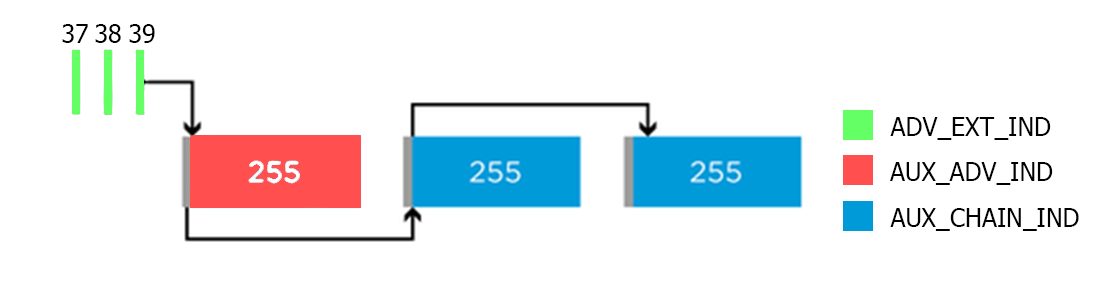
\includegraphics[width=0.7\textwidth]{./images/aux_chain_ind.png}
		\caption{Exemple de AUX\_CHAIN\_IND \cite{aux_chain_ind}}
		\label{fig:aux_chain_ind}
	\end{center}
\end{figure}

\subsection{Paràmetres}
BLE permet seleccionar qualsevol combinació de canals per on transmetre els anuncis.
Per consumir menys energia es pot transmetre en un únic canal però això es recomana no fer-ho ja que si el canal és sorollós el dispositius no es podrà detectar.
Tot i la flexibilitat

L'altre paràmetre molt important que es pot configurar és el interval d'anunci.
Aquest valor defineix el temps que passa entre que es transmeten anuncis pel mateix canal.
La especificació de BLE defineix que pot estar entre 20ms i 10.24s amb salts de 0.625ms.
Aquest paràmetre és crític depenent del servei que es vol oferir.
Si el valor és molt alt ajudarà a reduir el consum d'energia considerablement però això augmentarà la latència de transmissió de dades i de descobriment de dispositius.

Un cop s'estableix la connexió ja es poden enviar dades ràpidament però per establir la són necessaris múltiples intervals d'anunci i cal considerar que es possible que el receptor no detecti tots els anuncis. 
És per això que quan es desenvolupen serveis que interaccionen amb persones no és acceptable haver d'esperar desenes de segons per tant habitualment s'utilitzen valors d'entre 100 i 500 ms.
Per a dispositiu que requereixen la mínima latència possible en les dades s'utilitzen valors entre 20 i 50 ms.
Per últim, aquells dispositius que proporcionen dades que no varien sovint i que no requereixen interacció utilitzen valors des de 1 fins a 5 segons.

\begin{figure}[h!]
	\begin{center}
		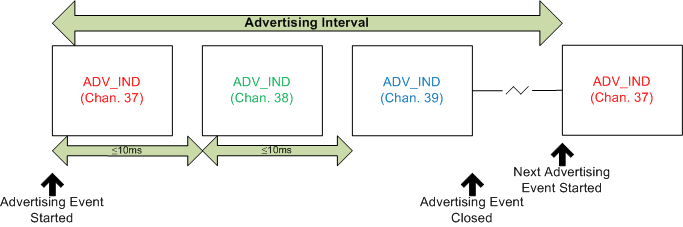
\includegraphics{./images/advertisement_params.png}
		\caption{Paràmetres d'anunci \cite{advertisment_params}}
		\label{fig:advertisment_params}
	\end{center}
\end{figure}

Tot i que es pot definir el valor del interval d'anunci cal tenir en compte que segons la especificació de BLE s'aplica un retard pseudo-aleatori que pot ser de fins a 10 ms i afecta als serveis que requereixen molt poca latència.

Tot i que fins ara s'ha parlat de definir un únic valor d'interval d'anunci habitualment s'estableix un règim on es va canviant aquest valor depenent de la situació.
Quan el dispositiu s'encén o quan s'espera una connexió es disminueix l'interval d'anunci per tal de que la connexió s'estableixi més ràpid.
En canvi, quan fa temps que no hi ha cap connexió s'augmenta l'interval d'anunci per reduir el consum d'energia. 


\section{Escaneig}
Quan un dispositius es vol anunciar a part de transmetre anuncis també ho pot fer fent escaneigs a dispositius que s'han anunciat prèviament.
La especificació de BLE 5 anomena el procés d'escanejar com a \textit{Device Discovery} i es basa en dos tipus, el escaneig actiu i el passiu.
En cas de fer escaneig passiu només es pot obtenir informació a través dels anuncis d'altres dispositius.
Si el escaneig és actiu es poden enviar requeriments d'escaneig per demanar informació addicional a la que hi ha als anuncis.

\subsection{Tipus}
En el cas dels paquets d'escaneig n'hi ha 2 originalment i BLE 5 n'afegeix 2 més.
El SCAN\_REQ serveix per requerir més informació a un dispositiu que s'està anunciant i que accepta aquest tipus de petició.
En el paquet no hi van dades pròpies, només s'hi indica el origen i destí.
El SCAN\_RSP és la resposta al paquet anterior, conté l'adreça pròpia del anunciador i fins a 31 bytes de dades.
La extensió que aporta BLE 5 defineix 2 nous tipus de paquets, el AUX\_SCAN\_REQ i el AUX\_SCAN\_RSP que tenen la mateixa funcionalitat que els anteriors respectivament.
La diferència és que serveixen per a quan es comunica a través de canals secundaris i que la quantitat de dades passa a ser de fins a 254 bytes en la resposta.

\subsection{Paràmetres}
El interval d'escaneig és el temps des de que es comença a escanejar en dos canals consecutius, es pot definir entre 10 ms i 10.24 s.
La finestra d'escaneig és el temps en que s'està escoltant a un canal.
Duració d'escaneig, és el temps que el dispositiu estarà escanejant.
Es pot configurar des de 10 ms fins a 65 segons o escaneig indefinit.
El període d'escaneig indica el temps entre que comencen les duracions d'escaneig i que serveix per poder fer pauses en que el dispositiu no escaneja.
Aquests paràmetres es poden identificar en la figura \ref{fig:escaneig_canals}.

%TODO: Refer gràfics
\begin{figure}[!h]
	\begin{center}
		\begin{subfigmatrix}{1}
			\subfigure[Escaneig de canals]{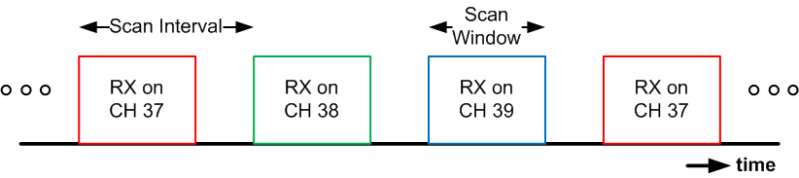
\includegraphics[width=0.8\textwidth]{./images/scanning_diagram}}
			\subfigure[Periodes de escaneig]{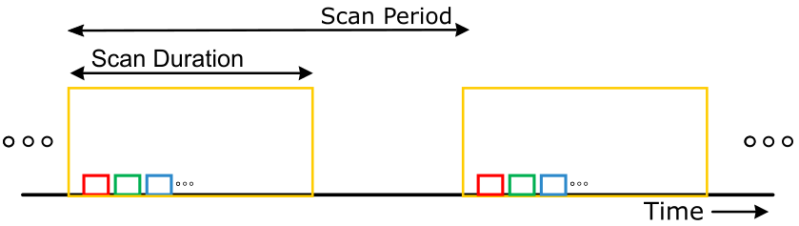
\includegraphics[width=0.8\textwidth]{./images/scanduationperiod}}
		\end{subfigmatrix}
	\end{center}
	\caption{Paràmetres d'escaneig}
	\label{fig:escaneig_canals}
\end{figure}

\section{Connexions}
S'ha vist com no cal establir una connexió per a transmetre poca informació.
Això permet desenvolupar implementacions molt simples per a situacions on es transmet amb molt poca freqüència. Tot i així, BLE també permet transmetre moltes més dades quan s'estableix una connexió.

Un cop s'hagui establert la connexió es podrà transmetre la informació molt eficientment, però establir la connexió suposa un cost energètic considerable.
Per tant alhora de definir els paràmetres de la connexió és important evitar, a ser possible, establir connexió cada vegada que es vol transmetre informació.

Com que les connexions estan basades en múltiples esdeveniments en instants determinats es considerà una connexió síncrona.
No hi ha limit de connexions segons l'especificació de BLE i per tant ve definit per les capacitats del dispositiu amb el que es treballa.

Per crear una connexió és necessari que un dispositiu tingui el rol GAP de central i un altre amb el rol de perifèric (els anunciadors i observadors no poden iniciar connexions).
%TODO: afegir referencia

El dispositiu central serà el que iniciarà la connexió i el perifèric el que l'acceptarà o no.
El central serà sempre el mestre i el perifèric serà el esclau de la connexió.
Per iniciar una connexió el mestre envia un missatge de tipus CONNECT\_IND\footnote{Aquest paquet en la versió 4 de BLE s'anomena CONNECT\_REQ} amb els paràmetres de la connexió.
En aquests paràmetres, tal i com es veurà més endavant, hi ha la informació necessària per determinar el primer esdeveniment de la connexió.
En cada esdeveniment els dos dispositius tenen un temps assignat per transmetre i per rebre dades.

\begin{figure}[h]
	\begin{center}
		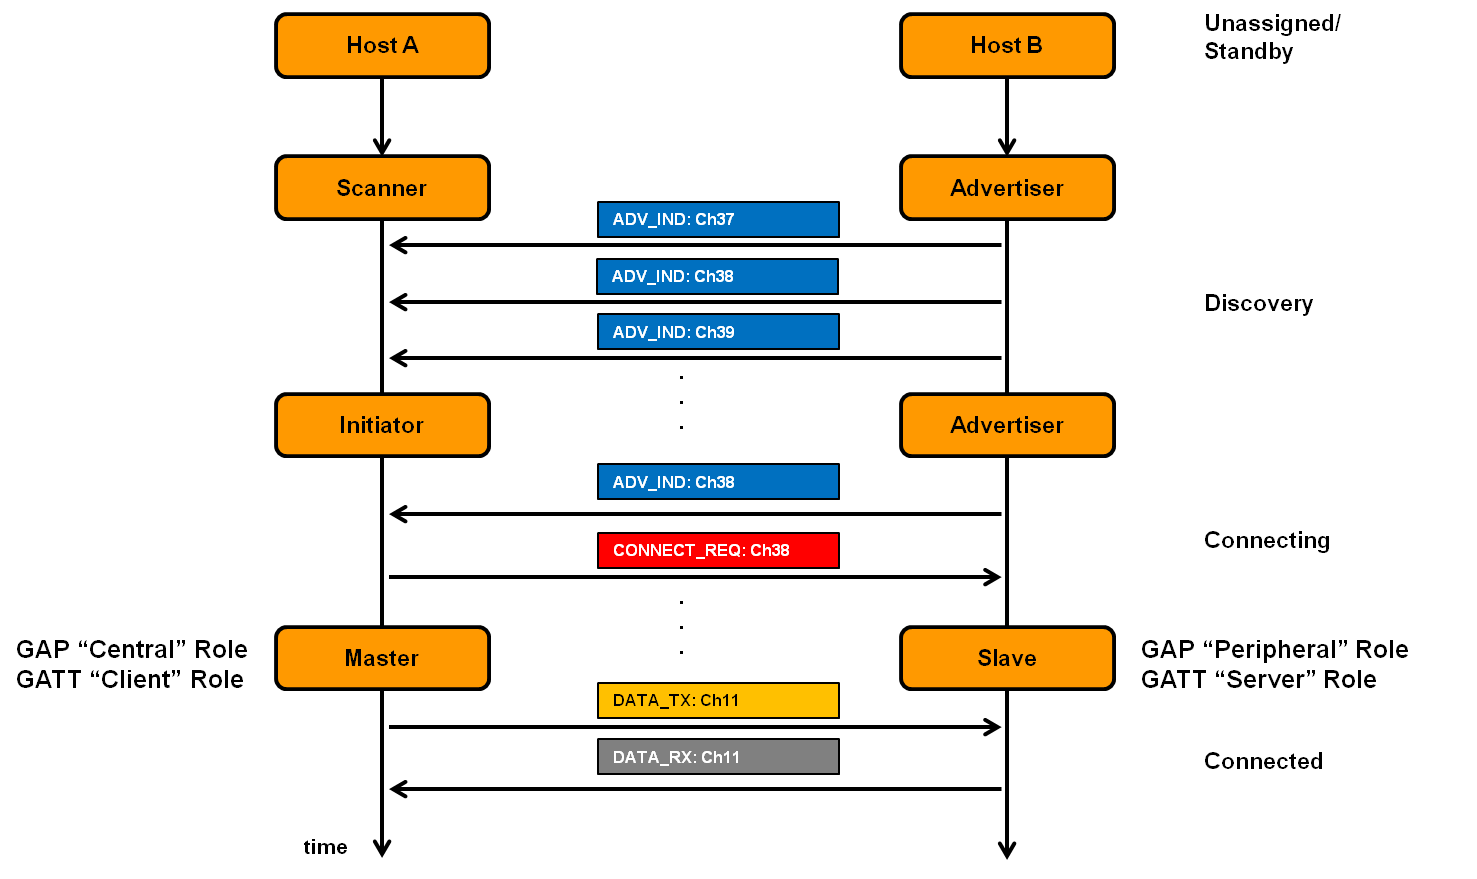
\includegraphics[width=1\textwidth]{./images/rols_unicast.png}
		\caption{Establiment de connexió}
	\end{center}
\end{figure}


En aquesta figura es pot veure el procediment en que dos dispositius estableixen una connexió.
Tenim el dispositiu A que inicialment està coma observador i el dispositiu B que s'està anunciant.
Cal recordar que els anuncis no es detecten tots ja que no sempre s'està transmetent i escoltant en el mateix canal.

El dispositiu A decideix establir una connexió amb el dispositiu B i envia un requeriment de connexió en l'últim canal en que s'ha escoltat l'anunci.
El dispositiu B després de transmetre un anunci per un canal escolta durant un temps determinat en el mateix canal a l'espera de requeriments de connexió.
Quan el dispositiu B rep el requeriment decideix acceptar la connexió respon al requeriment de connexió.

En aquest moment el dispositiu A passa a ser el mestre amb els rols Central i Client i el dispositiu B passa a ser l'esclau amb rols de perifèric i servidor.
La connexió està establerta i ja es possible transmetre dades entre ambdós dispositius durant els esdeveniments de connexió. 


\subsection{Paràmetres}
El interval de connexió és un dels paràmetres més importants en la connexió BLE, estableix com de sovint es comuniquen els dispositius.
És el temps que hi ha entre esdeveniments de la connexió i va entre 7.5 ms i 4 s.
Com que el que es configuren són preferències es determina l'interval mínim i el màxim que es vol.
En cas que es vulgui fixar simplement d'indica el mateix valor per al mínim i al màxim.

BLE permet al esclau saltar-se esdeveniments per tal d'estalviar bateria, per exemple si no te dades a transmetre.
La latència del esclau, que és un dels paràmetres de connexió, defineix la quantitat màxima de esdeveniments que l'esclau es pot saltar i que la connexió segueixi establerta.

%TODO: Refer gràfic
\begin{figure}[!h]
	\begin{center}
		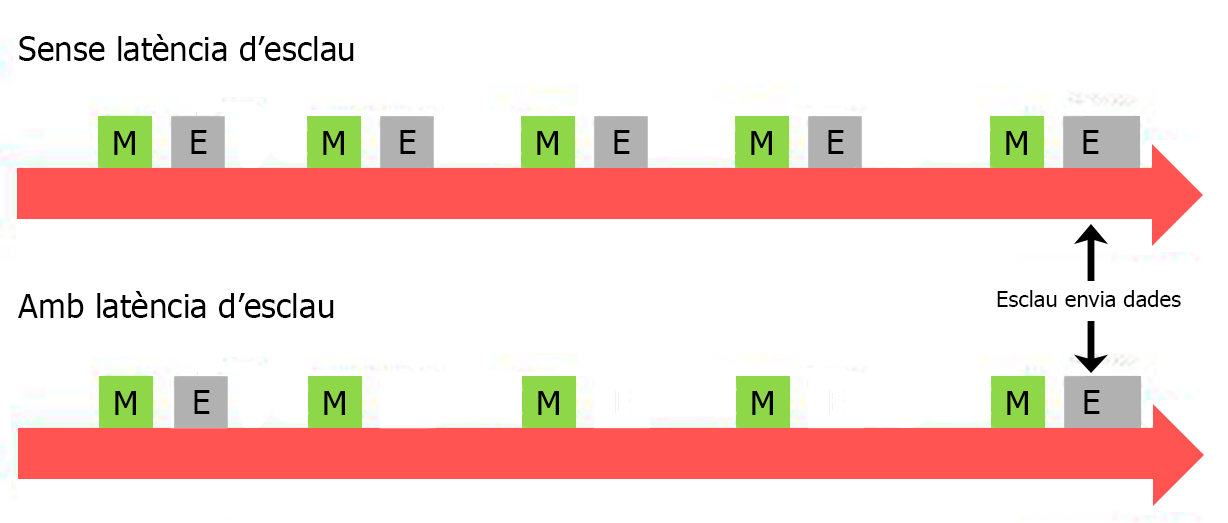
\includegraphics{./images/slave_latency_new.png}
		\caption{Comparació d'esdeveniments amb latència d'esclau \cite{slave_latency}}
	\end{center}
\end{figure}

L'últim paràmetre és el temps de supervisió, és el temps màxim acceptable que pot passar sense activitat en la connexió.
Si es supera aquest temps es considera que la connexió s'ha acabat i per tant per comunicar-se s'ha de tornar a iniciar.
Això pot passar per exemple en entorns molt sorollosos o més sovint quant els dispositius surten del seu abast i la senyal no és detectable.

\section{Seguretat}
\label{sec:security}
Com que l'ús de BLE és molt flexible per poder-lo utilitzar en certes aplicacions es requereix que l'intercanvi de dades sigui segur.
Això significa que la connexió tingui resistència a atacs de \textit{eavesdrop} passiu i de \textit{man in the middle}.
BLE utilitza l'encriptació simètrica AES-CCM, però la seguretat rau en com s'intercanvien la clau.

Hi ha diferents maneres que el desenvolupador pot escollir utilitzar i que varien en seguretat i facilitat d'ús.
Hi ha el mètode sense seguretat anomenat \textit{Just Works}.
Aquest mètode és útil en casos en que no es requereix seguretat o que no es possible tenir-ne per les limitacions del dispositiu amb el que es vol establir connexió.

Un altre mètode es el \textit{Out of Band} aquest permet utilitzar una altre tecnologia per l'intercanvi de claus.
Un exemple seria utilitzar NFC (comú en auriculars d'alta gama).
La seguretat d'aquest mètode depèn completament en el nou sistema per l'intercanvi de claus.

El més habitual és el \textit{Passkey} en que l'intercanvi de claus es bassa en una contrasenya de 4 a 6 dígits.
Cal tenir en compte que degut al baix número de combinacions depenent de la implementació aquest mètode serà sensible a atacs d'\textit{eavesdroping} passiu.

Finalment un mètode similar al anterior és el de Comparació Numèrica, enlloc de ser l'usuari qui introdueix el codi es genera automàticament i es mostra en els dos dispositius.
Cal comprovar que sigui el mateix número en els dos casos i això permet prevenir atacs de \textit{Man in the Middle} però de nou, no protegeix contra el \textit{Eavesdropping}.

\section{Format}
\label{sec:format}
En aquest apartat s'explicarà com estar format els paquets que s'envien en BLE i de quins camps està format.
Cal distingir però entre la versió 4 i la 5 de BLE ja que degut a les noves funcionalitats el format canvia considerablement.

\subsection{BLE 4.2}
En la versió de BLE 4.2\footnote{En les versions 4 i 4.1 la PDU tenia una mida màxima de 39 bytes.} els paquets que es transmeten tenen el següent format:

\begin{figure}[!h]
	\begin{center}
		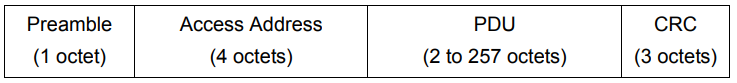
\includegraphics[width=1\textwidth]{./images/Packet_format_4_2.png}
		\caption{Format del paquet en BLE 4.2 \cite{BLE_4.2_packet_format}}
	\end{center}
\end{figure}

El preàmbul és una seqüència predefinida i que serveix per sincronisme.
L'adreça d'accés identifica a quina connexió pertany aquest paquet, en cas de ser d'anunci i no pertànyer a cap connexió el valor és 0x8E89BED6.
Aquest camp serveix al receptor per filtrar els paquets i només tractar aquells que interessa.
El CRC s'utilitza per detectar errors en el paquet. 

EN la PDU és on hi ha la informació pròpia del paquet i depenent de si és un paquet en un canal d'anunci o en un de dades té un format lleugerament diferent.

\begin{figure}[!h]
	\begin{center}
		\begin{subfigmatrix}{1}
			\subfigure[Format PDU d'anunci \cite{BLE_4.2_packet_format}]{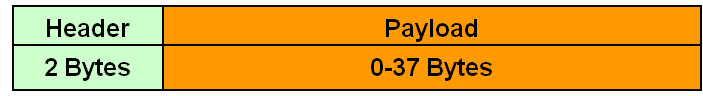
\includegraphics[width=0.8\textwidth]{./images/Packet_format_4_2_adv.png}}
			\subfigure[Format PDU de dades \cite{BLE_4.2_packet_format}]{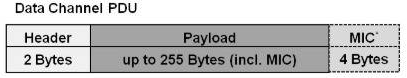
\includegraphics[width=0.8\textwidth]{./images/Packet_format_4_2_data.png}}
		\end{subfigmatrix}
	\end{center}
\end{figure}

Pel que fa a la PDU d'anunci és diferent segons el tipus de paquet.
En el cas del ADV\_IND està format per la adreça del anunciant seguit de un llistat d'estructures de dades d'anunci.
Aquestes estan formades per la longitud de la estructura, el tipus i les dades en si.
Hi ha molts tipus d'estructura que estan definits en el estàndard \cite{AD_Types}.

\begin{figure}[!h]
	\begin{center}
		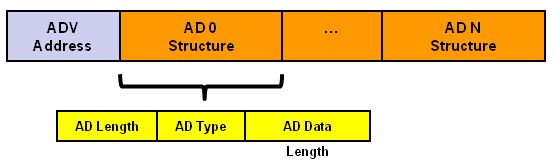
\includegraphics[width=0.8\textwidth]{./images/adv-ind-packet.png}
		\caption{Payload de ADV\_IND}
	\end{center}
\end{figure}

En canvi en el cas del ADV\_DIRECT\_IND simplement s'indica l'adreça del anunciador i la del dispositiu al que va dirigit el paquet.

\subsection{BLE 5}
Els canvis per a BLE 5 corresponen a les noves possibilitats que s'han comentat a \ref{Versions_BLE}.
Primer, la funcionalitat per poder transmetre anuncis als canals secundaris que s'ha comentat a \ref{Advertisement_Extensions} i enumerat els tipus de paquets a \ref{Advertising_Extension_PDU}.

\begin{figure}[!h]
	\begin{center}
		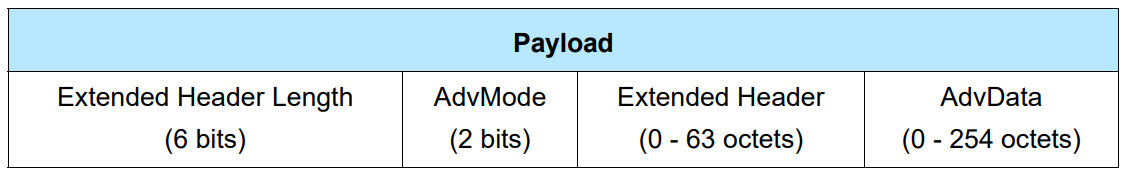
\includegraphics[width=0.8\textwidth]{./images/Common_Extended_Advertising_Payload_Format.png}
		\caption{Format de la Extended Advertising Payload \cite{BLE_5_Extended_Advertising}}
	\end{center}
\end{figure}

Tots els paquets nous de BLE 5 d'anunci es basen en aquest format flexible.
El \textit{Extended Header Length} defineix la longitud del \textit{Extended Header}.
El \textit{AdvMode} defineix una sèrie de valors que identifiquen si el anunciador accepta connexions o es pot escanejar.
El \textit{Extended Header} indica informació similar a la versió 4.2 com adreça del anunciador.
Però també indica tot allò necessari per BLE 5, com en quin canal secundari es transmetrà part de la informació del paquet o amb quin tipus de capa física es transmetrà aquesta informació (LE 1M, LE 2M o LE Coded) entre d'altres.
